\section{Probabilitat condicionada}

\textbf{Definició:} Siguin $A$ i $B$ dos successos d'un espai mostral $S$, amb $p(A) \neq 0$. S'anomena \textbf{probabilitat de $B$ condicionada a $A$} el quocient

\begin{equation}
p(B/A) = \frac{p(A\cap B)}{p(A)}
\end{equation}

Es llegeix: ``probabilitat del succés $B$ sabent que s'ha verificat el succés $A$''.

D'aquesta definició s'obtenen les \textbf{regles del producte}:

\begin{equation*}
p(A\cap B) = p(A)\cdot p(B/A) = p(B)\cdot p(A/B)
\end{equation*}

\textbf{Definició:} El succés $B$ és \textbf{independent} del succés $A$ si $p(B/A) = p(B)$. La relació és simètrica: si $B$ és independent de $A$, llavors $A$ és independent de $B$. En aquest cas:

\begin{equation}
p(A\cap B) = p(A)\cdot p(B)
\end{equation}

Si en canvi $p(A\cap B) \neq p(A)\cdot p(B)$, els successos són \textbf{dependents} i cal usar les fórmules de la probabilitat condicionada.

\section{Fórmula de Bayes}

Siguin $A_1, A_2, \ldots, A_k$ successos incompatibles dos a dos ($A_i\cap A_j = \varnothing$ per $i \neq j$) i exhaustius ($A_1\cup A_2\cup\cdots\cup A_k = \Omega$). Per a qualsevol succés $B$, el \textbf{teorema de la probabilitat total} dona:

\begin{equation*}
p(B) = p(A_1)\cdot p(B/A_1) + p(A_2)\cdot p(B/A_2) + \cdots + p(A_k)\cdot p(B/A_k)
\end{equation*}

La \textbf{fórmula de Bayes} permet calcular la probabilitat a posteriori de cada $A_j$ sabent que ha ocorregut $B$:

\begin{equation*}
p(A_j/B) = \frac{p(A_j)\cdot p(B/A_j)}{p(A_1)\cdot p(B/A_1) + p(A_2)\cdot p(B/A_2) + \cdots + p(A_k)\cdot p(B/A_k)}
\end{equation*}

\section{Variable aleatòria i funció de probabilitat}

\textbf{Definició:} Donat un espai mostral $\Omega$, una \textbf{variable aleatòria} $X$ és una aplicació

\begin{equation}
X: \Omega \to \mathbb{R}
\end{equation}

que assigna un nombre real a cada resultat possible de l'experiment.

Una variable aleatòria és \textbf{discreta} si el conjunt de valors que pot prendre és finit o numerable: $\{x_1, x_2, \ldots, x_n\}$.

\textbf{Definició:} La \textbf{funció de probabilitat} (o llei de probabilitat) d'una variable aleatòria discreta $X$ assigna a cada valor $x_i$ la seva probabilitat:

\begin{equation}
p[X = x_i] = p_i, \qquad \forall\, i = 1, 2, \ldots, n
\end{equation}

Ha de complir: $p_i \ge 0$ i $\displaystyle\sum_{i=1}^{n} p_i = 1$.

\section{Distribució binomial}

\textbf{Definició:} Una variable aleatòria $X$ segueix una \textbf{distribució binomial} $B(n, p)$ quan es realitza un experiment de Bernoulli (resultat èxit o fracàs, amb probabilitat d'èxit $p$) un total de $n$ proves independents. La funció de probabilitat és:

\begin{equation}
p[X = k] = \binom{n}{k}p^k(1-p)^{n-k} = \binom{n}{k}p^kq^{n-k}, \qquad k = 0, 1, \ldots, n
\end{equation}

on $q = 1 - p$.

Les condicions per aplicar la distribució binomial $B(n, p)$ són:

\begin{itemize}
\item El resultat de cada prova pertany a una de dues categories: èxit o fracàs.
\item La probabilitat d'èxit $p$ és constant en cada prova.
\item Les $n$ proves són independents entre si.
\end{itemize}

Les característiques principals de $B(n, p)$ són:

\begin{itemize}
\item \textbf{Esperança (mitjana):} $\mu = E[X] = np$
\item \textbf{Variància:} $\sigma^2 = npq = np(1-p)$
\item \textbf{Desviació típica:} $\sigma = \sqrt{npq}$
\end{itemize}

\section{Complement: distribució normal}

\subsection{Variable aleatòria contínua}

Una variable aleatòria contínua $X$ pot prendre qualsevol valor en un interval de $\mathbb{R}$. La seva distribució s'especifica mitjançant una \textbf{funció de densitat} $f(x) \ge 0$ tal que:

\begin{equation*}
\int_{-\infty}^{+\infty} f(x)\,dx = 1 \qquad\text{i}\qquad P(a \le X \le b) = \int_a^b f(x)\,dx
\end{equation*}

\subsection{La distribució normal $N(\mu, \sigma)$}

\textbf{Definició:} Una variable aleatòria $X$ segueix una \textbf{distribució normal} $N(\mu, \sigma)$ si la seva funció de densitat és

\begin{equation}
f(x) = \frac{1}{\sigma\sqrt{2\pi}}\,e^{-\frac{(x-\mu)^2}{2\sigma^2}}, \qquad x \in \mathbb{R}
\end{equation}

on $\mu$ és la mitjana i $\sigma$ la desviació típica.

\begin{figure}[H]
\centering
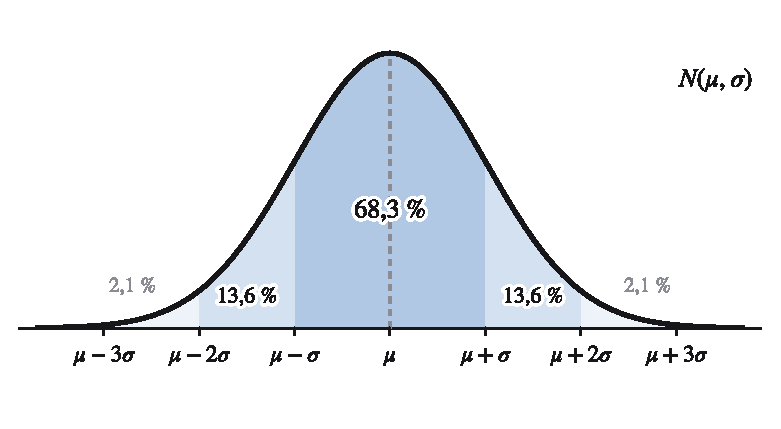
\includegraphics[width=372pt]{fig/m12_f26.pdf}
\caption{Campana de Gauss $N(\mu, \sigma)$: el 68,3 \% de les dades cau dins de $\mu \pm \sigma$, el 95,5 \% dins de $\mu \pm 2\sigma$ i el 99,7 \% dins de $\mu \pm 3\sigma$.}
\end{figure}

\subsection{Propietats de la distribució normal}

\begin{itemize}
\item La corba és simètrica respecte de $x = \mu$.
\item El punt de màxim és $x = \mu$, amb $f(\mu) = \dfrac{1}{\sigma\sqrt{2\pi}}$.
\item Els punts d'inflexió són $x = \mu \pm \sigma$.
\item $P(\mu - \sigma \le X \le \mu + \sigma) \approx 0{,}683$ \emph{(regla 68-95-99,7)}
\item $P(\mu - 2\sigma \le X \le \mu + 2\sigma) \approx 0{,}955$
\item $P(\mu - 3\sigma \le X \le \mu + 3\sigma) \approx 0{,}997$
\end{itemize}

\subsection{Tipificació: la normal estàndard $N(0, 1)$}

Per calcular probabilitats d'una $N(\mu, \sigma)$ qualsevol, es transforma en la normal estàndard $Z \sim N(0, 1)$ mitjançant el canvi de variable:

\begin{equation*}
Z = \frac{X - \mu}{\sigma}
\end{equation*}

\begin{equation*}
P(X \le x) = P\!\left(Z \le \frac{x - \mu}{\sigma}\right) = \Phi\!\left(\frac{x - \mu}{\sigma}\right)
\end{equation*}

on $\Phi(z)$ és la funció de distribució acumulada de la normal estàndard, consultable en taules.

\textbf{Propietat (Simetria de $\Phi$):} per a la normal estàndard es compleix

\begin{equation}
P(Z \le -z) = 1 - P(Z \le z) = 1 - \Phi(z)
\end{equation}

\begin{equation}
P(Z \ge z) = 1 - \Phi(z)
\end{equation}

\begin{equation}
P(a \le Z \le b) = \Phi(b) - \Phi(a)
\end{equation}

\subsection{Aproximació binomial--normal}

Quan $n$ és gran i $p$ no és molt proper a $0$ ni a $1$, la distribució $B(n, p)$ s'aproxima a:

\begin{equation*}
X \sim B(n, p) \approx N(\mu, \sigma) \quad\text{amb}\quad \mu = np, \quad \sigma = \sqrt{npq}
\end{equation*}

\emph{Regla pràctica:} aplicar quan $np \ge 5$ i $nq \ge 5$.

\section{Complement: probabilitat bàsica, taules i arbres}

\subsection{Regla de Laplace i operacions amb successos}

Si tots els resultats són \textbf{equiprobables}:

\begin{equation*}
P(A)=\frac{\text{casos favorables}}{\text{casos possibles}}
\end{equation*}

\begin{table}[H]
\centering
\renewcommand{\arraystretch}{1.25}
\begin{tabular}{lc}
\toprule
Operació & Fórmula \\
\midrule
Contrari & $P(\overline A)=1-P(A)$ \\
Unió & $P(A\cup B)=P(A)+P(B)-P(A\cap B)$ \\
Intersecció (producte) & $P(A\cap B)=P(A)\,P(B\mid A)$ \\
Independents & $P(A\cap B)=P(A)\,P(B)$ \\
Lleis de De Morgan & $P(\overline{A\cup B})=P(\overline A\cap\overline B)$, $\ P(\overline{A\cap B})=P(\overline A\cup\overline B)$ \\
\bottomrule
\end{tabular}
\end{table}

\begin{figure}[H]
\centering
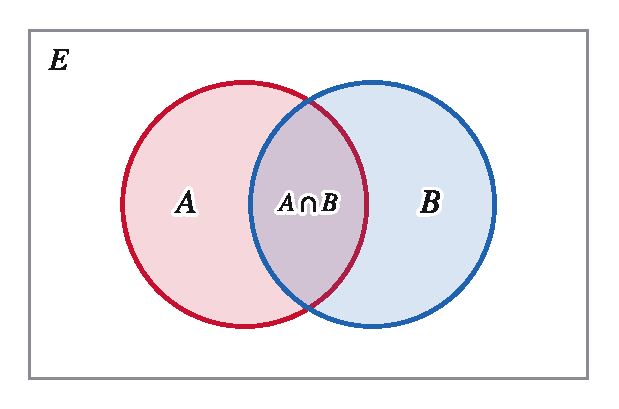
\includegraphics[width=297pt]{fig/m12_f38.pdf}
\caption{Diagrama de Venn de dos successos $A$ i $B$ dins de l'espai mostral $E$.}
\end{figure}

\emph{Exemple:} $P(A)=0{,}5$, $P(B)=0{,}4$ i $P(A\cup B)=0{,}7$. Llavors $P(A\cap B)=0{,}5+0{,}4-0{,}7=0{,}2$. Com que $P(A)P(B)=0{,}2$, \textbf{$A$ i $B$ són independents}.

\subsection{Taules de contingència}

Una taula de doble entrada permet llegir directament les probabilitats.

\begin{table}[H]
\centering
\renewcommand{\arraystretch}{1.25}
\begin{tabular}{lccc}
\toprule
 & $B$ & $\overline B$ & Total \\
\midrule
$A$ & 30 & 20 & 50 \\
$\overline A$ & 10 & 40 & 50 \\
Total & 40 & 60 & 100 \\
\bottomrule
\end{tabular}
\end{table}

$P(A\cap B)=\frac{30}{100}$, $P(B)=\frac{40}{100}$ i $P(A\mid B)=\dfrac{30}{40}=0{,}75$ (es divideix per la fila o columna de la condició).

\subsection{Diagrames d'arbre, probabilitat total i Bayes}

Les probabilitats de les branques d'una mateixa ramificació sumen $1$. El producte de les branques d'un camí és la probabilitat de la intersecció; sumant camins s'obté la \textbf{probabilitat total}.

\begin{figure}[H]
\centering
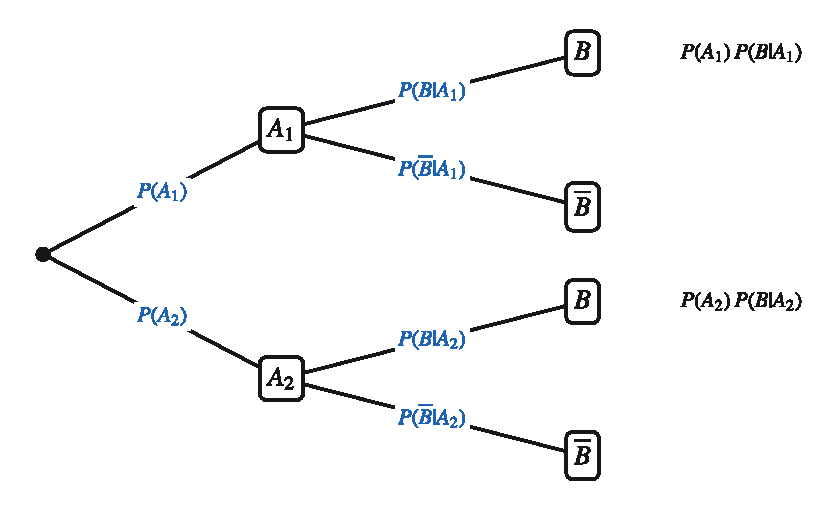
\includegraphics[width=372pt]{fig/m12_f39.pdf}
\caption{Arbre de probabilitats: $P(B)=P(A_1)P(B|A_1)+P(A_2)P(B|A_2)$.}
\end{figure}

\emph{Exemple:} Una fàbrica té dues màquines: $M_1$ fa el $60\,\%$ de les peces, amb un $2\,\%$ de defectuoses, i $M_2$ fa el $40\,\%$, amb un $5\,\%$ de defectuoses.

\begin{equation*}
P(D)=0{,}6\cdot0{,}02+0{,}4\cdot0{,}05=0{,}012+0{,}02=0{,}032
\end{equation*}

Si una peça és defectuosa, la probabilitat que vingui de $M_2$ és (Bayes)

\begin{equation*}
P(M_2\mid D)=\frac{0{,}4\cdot0{,}05}{0{,}032}=\frac{0{,}02}{0{,}032}=0{,}625
\end{equation*}

\section{Complement: esperança, variància i exemples resolts}

\subsection{Esperança i variància}

Per a una variable aleatòria discreta amb valors $x_i$ i probabilitats $p_i$:

\begin{equation*}
\mu=E[X]=\sum x_i\,p_i,\qquad \operatorname{Var}(X)=\sum x_i^2\,p_i-\mu^2,\qquad \sigma=\sqrt{\operatorname{Var}(X)}
\end{equation*}

\emph{Exemple:} Un joc paga $10$ \euro{} amb probabilitat $0{,}1$, $2$ \euro{} amb probabilitat $0{,}4$ i $0$ \euro{} amb probabilitat $0{,}5$.

\begin{equation*}
E[X]=10\cdot0{,}1+2\cdot0{,}4=1{,}8\text{ €},\qquad \operatorname{Var}(X)=100\cdot0{,}1+4\cdot0{,}4-1{,}8^2=11{,}6-3{,}24=8{,}36
\end{equation*}

Per a $B(n,p)$: $E[X]=np$ i $\operatorname{Var}(X)=npq$.

\subsection{Binomial resolta}

Es llança $5$ cops una moneda trucada amb $P(\text{cara})=0{,}6$. Probabilitat d'obtenir \textbf{exactament} $3$ cares i d'obtenir \textbf{almenys} $1$:

\begin{equation*}
P(X=3)=\binom53 0{,}6^3\,0{,}4^2=10\cdot0{,}216\cdot0{,}16=0{,}3456
\end{equation*}

\begin{equation*}
P(X\ge1)=1-P(X=0)=1-0{,}4^5=1-0{,}01024=0{,}98976
\end{equation*}

\subsection{Normal resolta amb tipificació}

Les notes d'un examen segueixen $N(6;\,1{,}5)$. Percentatge d'alumnes amb nota superior a $8$:

\begin{equation*}
P(X>8)=P\!\left(Z>\frac{8-6}{1{,}5}\right)=P(Z>1{,}33)=1-\Phi(1{,}33)=1-0{,}9082=0{,}0918
\end{equation*}

És a dir, un $9{,}18\,\%$ aproximadament. Per a un interval: $P(5\le X\le7)=P(-0{,}67\le Z\le0{,}67)=2\Phi(0{,}67)-1=2\cdot0{,}7486-1=0{,}4972$.

\subsection{Binomial aproximada per la normal}

$X\sim B(100;\,0{,}5)$: $np=50\ge5$, $nq=50\ge5$, de manera que $X\approx N(50;\,5)$ amb $\sigma=\sqrt{100\cdot0{,}5\cdot0{,}5}=5$.

$P(X\le55)$: amb \textbf{correcció de continuïtat} es calcula $P(X'\le55{,}5)$:

\begin{equation*}
P\!\left(Z\le\frac{55{,}5-50}{5}\right)=P(Z\le1{,}1)=\Phi(1{,}1)=0{,}8643
\end{equation*}
